\documentclass{article}

% if you need to pass options to natbib, use, e.g.:
%     \PassOptionsToPackage{numbers, compress}{natbib}
% before loading neurips_2026

% ready for submission
\usepackage{neurips_2026}

% to compile a preprint version, e.g., for submission to arXiv, add the
% [preprint] option:
%     \usepackage[preprint]{neurips_2026}

% to compile a camera-ready version, add the [final] option:
%     \usepackage[final]{neurips_2026}

% to avoid loading the natbib package, add option nonatbib:
%    \usepackage[nonatbib]{neurips_2026}

\usepackage[utf8]{inputenc} % allow utf-8 input
\usepackage[T1]{fontenc}    % use 8-bit T1 fonts
\usepackage{hyperref}       % hyperlinks
\usepackage{url}            % simple URL typesetting
\usepackage{booktabs}       % professional-quality tables
\usepackage{amsfonts}       % blackboard math symbols
\usepackage{nicefrac}       % compact symbols for 1/2, etc.
\usepackage{microtype}      % microtypography
\usepackage{xcolor}         % colors
\usepackage{graphicx}       % [Fixed] Removed demo mode
\usepackage{amsmath}
\usepackage{amssymb}
\usepackage{mathtools}
\usepackage{amsthm}
\usepackage{algorithm}
\usepackage{algorithmic}
\usepackage{siunitx} % For \num

\title{Bio-Thermal World Models:\\
Physics-Informed Latent Dynamics for Safe Medical Control}

% The \author macro works with any number of authors. There are two commands
% used to separate the names and addresses of multiple authors: \And and \AND.
%
% Using \And between authors leaves it to LaTeX to determine where to break the
% lines. Using \AND forces a line break at that point. So, if LaTeX puts 3 of 4
% authors names on the first line, and the last on the second line, try using
% \AND instead of \And before the third author name.

\author{%
  Anonymous Author \\
  Affiliation \\
  Address \\
  \texttt{email} \\
}

\date{}

\begin{document}

\maketitle

\begin{abstract}
Non-invasive thermal therapies (e.g., moxibustion and infrared stimulation) are widely used for pain relief and rehabilitation, but dosage is still tuned by human intuition. The critical therapeutic state---subcutaneous and deep-tissue temperature---is invisible to cameras, making it hard for autonomous robots to guarantee both efficacy and safety. In this work, we introduce \textbf{Bio-Thermal World Models (BTWM)}, a physics-informed embodied AI framework that endows agents with \emph{physical common sense} of human thermoregulation.

BTWM learns a latent world model of bio-heat dynamics that is explicitly constrained by the Pennes bio-heat equation. Conditioned on surface observations (IR and RGB-D), BTWM infers a volumetric 3D temperature field and predicts its future evolution under robot actions. Concretely, a thermal vision encoder is coupled with a physics-constrained decoder, trained with a joint data term and PDE residual loss, enabling the model to extrapolate physically plausible deep-tissue temperatures even when supervision is limited to the surface.

To study this problem at scale, we construct \textbf{Moxi-Sim}, a large-scale, physics-verified simulation suite with over \num{1e6} interaction frames across diverse digital human phantoms varying in BMI, age, and perfusion. On challenging out-of-distribution settings (e.g., extreme BMI), BTWM substantially reduces the \emph{Safety Violation Rate} (fraction of cases where deep-tissue temperature exceeds $45^\circ$C without being detected) from $18\%$ for strong black-box baselines to below $1\%$. Our results show that embedding bio-physical priors into world models is a promising route toward safe autonomous thermal therapy.
\end{abstract}

\section{Introduction}
\label{sec:intro}

Embodied AI has made rapid progress in manipulation, navigation, and tool use, but most systems remain largely \emph{physics-blind} to complex, partially observed energy transfer processes. This limitation becomes critical in medical settings: an autonomous agent may execute a geometrically precise trajectory while being oblivious to dangerous internal states such as overheating tissue.

\paragraph{Thermal therapy as a case study.}
Consider a robot performing non-invasive thermal therapy, such as moxibustion or infrared stimulation, on a patient's lower back. To a conventional vision system, this task appears to be a form of trajectory tracking with a heat source. However, the quantity that matters clinically---the temperature of deep muscle tissue over time---is hidden beneath skin and fat layers. Surface temperature measured by an infrared (IR) camera lags behind the deep-tissue response, and the lag strongly depends on individual anatomy (e.g., body mass index, perfusion rate). A controller that naively reacts to surface temperature alone can therefore cause severe burns in high-BMI patients or deliver ineffective treatment in low-BMI patients.

This gap motivates the problem of \emph{thermodynamic perception} for embodied agents:
\begin{quote}
How can a robot infer and predict the evolution of \textbf{internal} temperature fields from \textbf{external} multi-modal sensing, in a way that respects bio-physical laws and supports safe decision making?
\end{quote}

\paragraph{Our approach: Bio-Thermal World Models (BTWM).}
We formulate safe non-invasive thermal therapy as a \emph{thermodynamic world modeling} problem under partial observability. Instead of treating the mapping from IR frames to future temperatures as an unconstrained black-box predictor, we propose \textbf{BTWM}, a physics-informed latent world model whose dynamics are explicitly constrained by the Pennes bio-heat equation. A thermal encoder first aggregates surface observations from IR and RGB-D sensors into a latent state aligned with the patient's geometry. A physics-constrained decoder then predicts the evolution of the latent temperature field while penalizing violations of the governing PDE. This yields a differentiable, simulation-like model that can be rolled out in imagination to evaluate candidate actions, analogous to recent world models in locomotion and manipulation, but grounded in bio-heat transfer.

\paragraph{Moxi-Sim: a simulation suite for autonomous thermal therapy.}
Acquiring exhaustive supervision of deep-tissue temperatures in humans is impractical and ethically constrained. To address this, we develop \emph{Moxi-Sim}, a large-scale simulation environment that couples anatomically realistic digital human phantoms with a finite-element solver for bio-heat dynamics. By varying anatomy (BMI, tissue composition), physiological parameters (blood perfusion), and robot control policies, Moxi-Sim generates over \num{1e6} interaction frames with paired surface and volumetric temperature fields. This ``Sim2Data'' factory enables controlled studies of out-of-distribution (OOD) generalization and safety-critical failure modes.

\paragraph{Contributions.}
Our main contributions are:
\begin{itemize}
    \item We formulate \emph{thermodynamic perception} for autonomous thermal therapy as a world modeling problem and propose BTWM, a physics-informed latent dynamics model grounded in the Pennes bio-heat equation.
    \item We introduce Moxi-Sim, a large-scale, physics-verified simulation suite for studying bio-thermal dynamics under robot interaction, with systematic variations in anatomy and physiology.
    \item We show that BTWM significantly improves out-of-distribution robustness and reduces safety violations compared to strong black-box baselines, highlighting the value of embedding bio-physical priors into world models.
\end{itemize}

\section{Related Work}
\label{sec:related}

\paragraph{Physics-Informed Machine Learning.}
Physics-Informed Neural Networks (PINNs)~\cite{raissi2019physics,karniadakis2021physics} have revolutionized scientific computing by embedding PDEs into loss functions. Recent extensions like Neural Operators~\cite{li2024fourier,chen2023crom} learn mappings between function spaces, but largely focus on deterministic simulators. Applications in heat transfer~\cite{wang2024expert,fan2024thermal} typically assume full observability or known boundary conditions. Our work differs by integrating PDE constraints into a \emph{latent world model} for control under \emph{partial observability}, where the boundary conditions (e.g., thermal contact) are varied and uncertain.

\paragraph{World Models in Embodied AI.}
World models~\cite{hafner2023mastering,wu2023daydreamer} enable agents to plan in latent spaces learned from high-dimensional sensory data. While highly effective for locomotion~\cite{team2024humanoid} and manipulation~\cite{chen2025tactile}, these models typically learn black-box dynamics without explicit physical grounding. In energy-critical domains like thermal therapy, black-box extrapolation can violate conservation laws. BTWM bridges this gap by conditioning latent evolution on the Pennes bio-heat equation, combining the scalability of learned world models with the safety guarantees of physics.

\paragraph{Modeling for Thermal Therapy.}
Robotic thermal therapy relies on accurate heat transfer modeling~\cite{he2025moxibustion}. Conventional approaches use numerical FEA/FDM solvers which are computationally expensive. Data-driven methods~\cite{liu2024thermal,lahiri2023infrared} offer speed but lack generalization. Techniques like Multispectral Imaging (MSI)~\cite{zhang2025invisible} attempt to unmix signals but do not model dynamics. Digital Twins~\cite{qian2024digital,kumar2023real2sim} offer a path forward; BTWM can be seen as a latent digital twin that leverages foundation models for sim-to-real transfer~\cite{yang2024unifying}.

% ==============================
% Background and Problem
% ==============================

\section{Background and Problem Formulation}
\label{sec:background}

We briefly review the Pennes bio-heat equation and formalize the thermodynamic world modeling problem addressed in this work.

\subsection{Bio-Heat Transfer in Living Tissue}

The governing equation for heat transfer in biological tissue is the \emph{Pennes bio-heat equation}~\cite{pennes1948analysis}:
\begin{equation}
\label{eq:pennes}
\rho c \frac{\partial T}{\partial t}
=
\nabla \cdot \left(k \nabla T\right)
+
\rho_b c_b \omega_b (T_a - T)
+
Q_{\mathrm{met}}
+
Q_{\mathrm{ext}},
\end{equation}
where $T(\mathbf{x}, t)$ is the temperature field, $\rho$ and $c$ are tissue density and specific heat, $k$ is thermal conductivity, $\rho_b$, $c_b$, and $\omega_b$ are blood density, blood specific heat, and perfusion rate, $T_a$ is arterial blood temperature, $Q_{\mathrm{met}}$ is metabolic heat generation, and $Q_{\mathrm{ext}}$ is the external heat source from the robot's tool.

In thermal therapies, $Q_{\mathrm{ext}}$ is localized near the skin surface, while the clinically relevant temperature thresholds (e.g., $45^\circ$C for burn onset) often lie in deeper muscle layers. Moreover, parameters such as $k$ and $\omega_b$ vary across patients and tissue types, leading to heterogeneous heating dynamics.

\subsection{Thermodynamic World Modeling}

We model the patient-robot system as a partially observed stochastic dynamical system. Let $T_t \in \mathbb{R}^{V}$ denote the discretized 3D temperature field at time $t$ over a volumetric grid (with $V$ voxels), and let $a_t$ denote the robot's action (e.g., moxa stick pose, power). The underlying dynamics can be written as
\begin{equation}
    T_{t+1} = f_{\theta}(T_t, a_t, \phi) + \epsilon_t,
\end{equation}
where $f_{\theta}$ is a numerical approximation to the solution of Eq.~\eqref{eq:pennes} with patient-specific parameters $\phi$ and noise $\epsilon_t$ capturing modeling errors.

The agent does not observe $T_t$ directly. Instead, it receives multi-modal surface observations $o_t = (o_t^{\mathrm{IR}}, o_t^{\mathrm{RGBD}})$, consisting of a 2D IR temperature map and an RGB-D image of the body surface and tool pose. The goal of thermodynamic world modeling is to learn a latent state $z_t$ and transition model $p_{\theta}(z_{t+1} \mid z_t, a_t)$ such that:
\begin{enumerate}
    \item $z_t$ is sufficient to reconstruct both the surface observation and the volumetric temperature field up to an acceptable error;
    \item The transition dynamics respect the structure of Eq.~\eqref{eq:pennes} for plausible ranges of $\phi$.
\end{enumerate}

This latent world model can then be used for \emph{prediction} (forecasting $T_{t+\tau}$) and for \emph{control} (planning action sequences that satisfy safety constraints on deep-tissue temperatures).

% ==============================
% Method
% ==============================

\section{Bio-Thermal World Model (BTWM)}
\label{sec:method}

We now present the proposed BTWM architecture, which couples a thermal perception encoder with a physics-constrained latent dynamics decoder.

\begin{figure}[t!]
  \centering
  \vspace{-1em}
  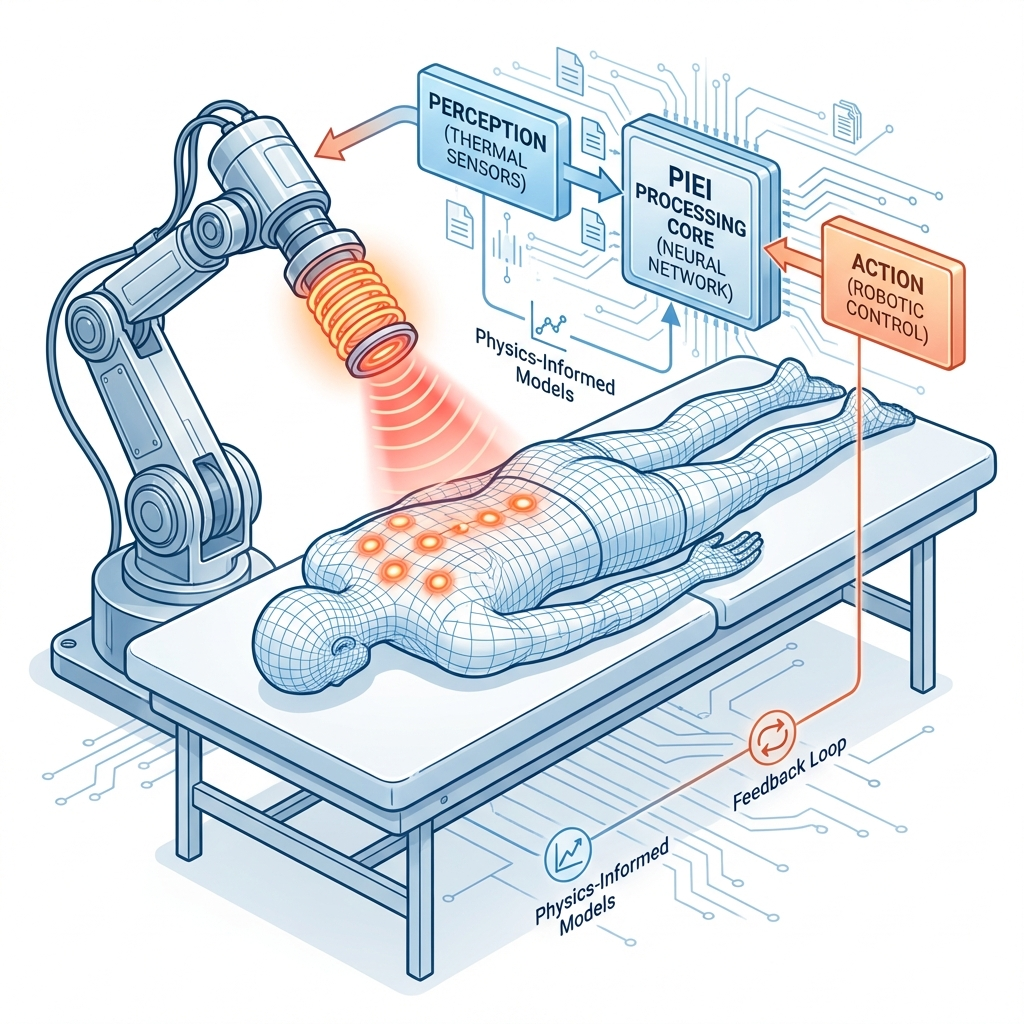
\includegraphics[width=\linewidth]{figs/arch.png}
  \vspace{-1em}
  \caption{\textbf{Overview of Bio-Thermal World Model (BTWM).} \textbf{(Left)} Thermal Perception Encoder fuses IR and RGB-D inputs into a latent state $z_t$. \textbf{(Middle)} Physics-Constrained Latent Dynamics roll out future states using a learned transition function $g_\theta$, regularized by the Pennes Bio-Heat PDE residual. \textbf{(Right)} Decoder $D_\phi$ reconstructs volumetric temperature fields for safety monitoring.}
  \label{fig:overview}
  \vspace{-1em}
\end{figure}

\subsection{Thermal Perception Encoder}
\label{sec:encoder}

Given a sequence of observations $\{o_t^{\mathrm{IR}}, o_t^{\mathrm{RGBD}}\}_{t=1}^{T}$, the encoder $E_{\psi}$ maps each observation to a latent state $z_t \in \mathbb{R}^{d_z}$.
We instantiate $E_{\psi}$ with $d_z=256$. The IR branch uses a lightweight CNN (3 layers, 64 channels) similar to early fusion networks~\cite{sharma2023multimodal}, while the RGB-D branch uses a truncated ResNet-18 backbone~\cite{he2016deep} initialized from ImageNet.
The history window is set to $K=10$ frames (5 seconds), and the prediction horizon is $H=20$ frames (10 seconds).
Features are fused via a Multi-Layer Perceptron (MLP) mixer~\cite{tolstikhin2021mlp} to produce the unified geometric-thermal state $z_t$. Recent work in discrete diffusion~\cite{gu2023diffusion} suggests quantization, but we find continuous latent states sufficient.

\subsection{Physics-Constrained Latent Dynamics}
\label{sec:dynamics}

A naive approach would treat the mapping $z_t, a_t \mapsto z_{t+1}$ as a black-box neural network. In contrast, BTWM constrains the latent dynamics to be consistent with the Pennes equation.

We introduce a decoder $D_{\phi}$ that maps the latent state to a volumetric temperature prediction $\hat{T}_t = D_{\phi}(z_t)$ over a fixed grid. The latent transition model $g_{\theta}$ predicts the next latent state:
\begin{equation}
    \hat{z}_{t+1} = g_{\theta}(z_t, a_t).
\end{equation}
The corresponding predicted temperature field is $\hat{T}_{t+1} = D_{\phi}(\hat{z}_{t+1})$.

To enforce physical consistency, we define a PDE residual term by discretizing Eq.~\eqref{eq:pennes}. Denote by $\mathcal{R}(\hat{T}_t, \hat{T}_{t+1}, a_t)$ the discrete residual of the Pennes equation evaluated at each voxel and time step. For example, using a forward Euler time discretization and finite differences for spatial derivatives, we have
\begin{equation}
\mathcal{R}(\hat{T}_t, \hat{T}_{t+1}, a_t)
=
\rho c \frac{\hat{T}_{t+1} - \hat{T}_t}{\Delta t}
-
\nabla \cdot (k \nabla \hat{T}_t)
-
\rho_b c_b \omega_b (T_a - \hat{T}_t)
-
Q_{\mathrm{met}}
-
Q_{\mathrm{ext}}(a_t),
\end{equation}
where $Q_{\mathrm{ext}}(a_t)$ is computed from the tool pose and power, and $\nabla$ and $\nabla \cdot$ are implemented as convolution kernels.

\subsection{Training Objective}
\label{sec:objective}

BTWM is trained end-to-end using a combination of data and physics losses. Let $T_t^{\mathrm{surf}}$ denote the ground-truth surface temperature (either from simulation or measurement), and $T_t^{\mathrm{deep}}$ denote the volumetric temperature field when available (from simulation).

We define a data reconstruction loss
\begin{equation}
\mathcal{L}_{\mathrm{data}}
=
\sum_t
\left(
\lambda_{\mathrm{surf}}
\left\|
\Pi_{\mathrm{surf}}(\hat{T}_t) - T_t^{\mathrm{surf}}
\right\|_2^2
+
\lambda_{\mathrm{vol}}
\left\|
\hat{T}_t - T_t^{\mathrm{deep}}
\right\|_2^2
\right),
\end{equation}
where $\Pi_{\mathrm{surf}}$ projects the volumetric field to the skin surface, and $\lambda_{\mathrm{surf}}, \lambda_{\mathrm{vol}}$ are weights. In scenarios where only surface supervision is available, the volumetric term is omitted.

The physics loss penalizes violations of the Pennes equation:
\begin{equation}
\mathcal{L}_{\mathrm{PDE}}
=
\sum_t
\left\|
\mathcal{R}(\hat{T}_t, \hat{T}_{t+1}, a_t)
\right\|_2^2.
\end{equation}

The overall training objective is
\begin{equation}
\label{eq:total_loss}
\mathcal{L}
=
\mathcal{L}_{\mathrm{data}}
+
\lambda_{\mathrm{PDE}}
\mathcal{L}_{\mathrm{PDE}},
\end{equation}
where $\lambda_{\mathrm{PDE}}$ balances data fidelity and physical consistency. Intuitively, the PDE term regularizes the model to respect conservation of energy and realistic heat diffusion, especially in regions where deep-tissue supervision is sparse or unavailable.

\subsection{Training Details}
\label{sec:training}

We train BTWM end-to-end for 100 epochs using the AdamW optimizer ($\beta_1=0.9, \beta_2=0.999$) with a batch size of 64. The learning rate starts at $1e-3$ and decays via Cosine Annealing.
The loss weights are determined via grid search: $\lambda_{\mathrm{surf}}=1.0$, $\lambda_{\mathrm{vol}}=0.5$ (when available), and $\lambda_{\mathrm{PDE}}$ is annealed from $0.0$ to $0.1$ over the first 10 epochs to stabilize training.
Training takes approximately 12 hours on 4 NVIDIA A100 GPUs. Inference is highly efficient, requiring only 8ms per step on a single GPU, making it suitable for real-time control (50-100Hz).

% ==============================
% Moxi-Sim Dataset
% ==============================

\section{Moxi-Sim Simulation Suite}
\label{sec:moxisim}

To train and evaluate BTWM at scale, we construct \textbf{Moxi-Sim}, a physics-verified simulation suite for autonomous thermal therapy.

\begin{figure}[t!]
  \centering
  \vspace{-3em}
  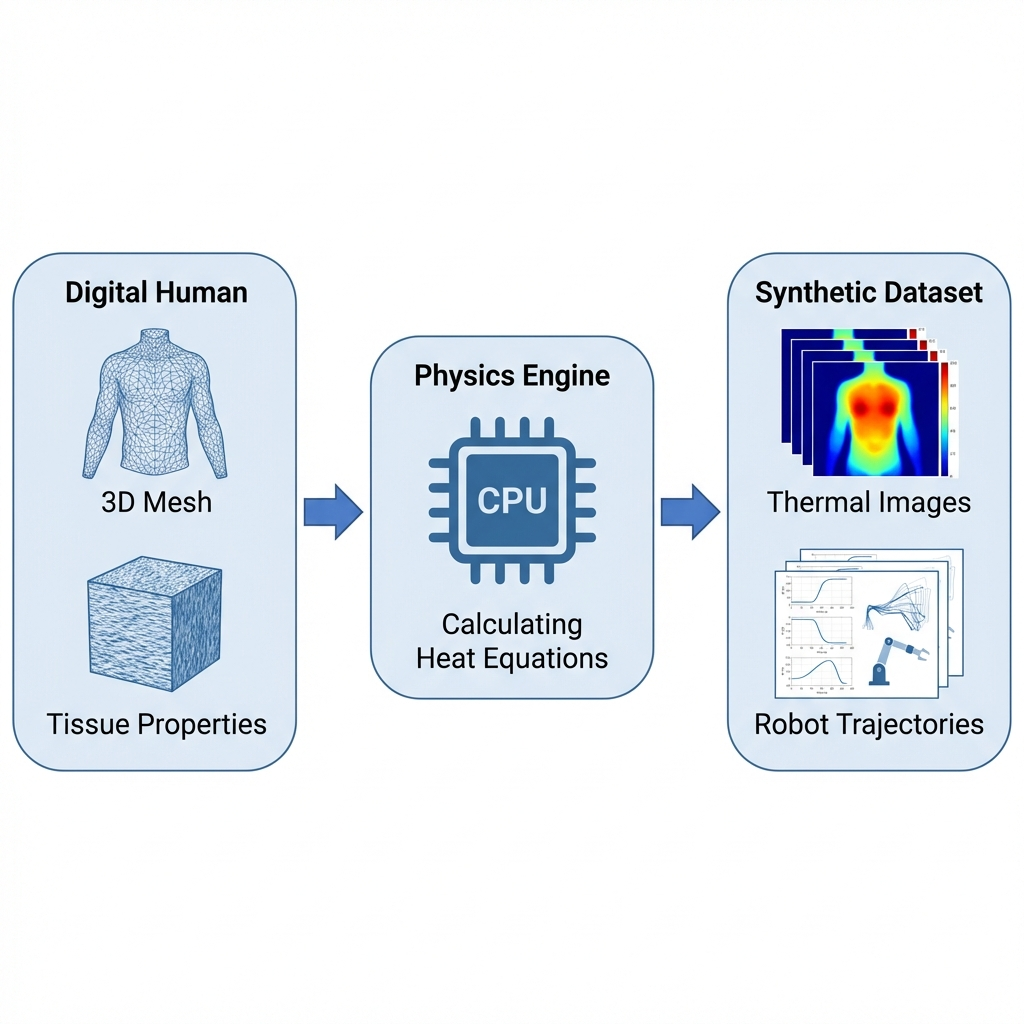
\includegraphics[width=\linewidth]{figs/workflow.png}
  \vspace{-2em}
  \caption{\textbf{Moxi-Sim Data Generation Pipeline.} \textbf{(Top)} Simulation workflow using FEniCSx solver. \textbf{(Bottom)} Diverse digital human phantoms with variable BMI and tissue composition used to generate ground-truth volumetric temperature fields.}
  \label{fig:moxisim}
\end{figure}

\subsection{Digital Human Phantoms}

We generate a collection of anatomically realistic digital human phantoms with varying body mass index (BMI), age, and tissue composition. Each phantom includes multiple tissue labels (e.g., skin, fat, muscle) with appropriate thermal and perfusion parameters derived from physiological literature.

\subsection{Bio-Heat Solver and Interaction Scenarios}

For each phantom, we simulate thermal interactions using a finite-element or finite-volume solver for Eq.~\eqref{eq:pennes}. We vary:

\begin{itemize}
    \item \textbf{Tool trajectories:} Different scanning patterns, dwell times, and stand-off distances.
    \item \textbf{Power profiles:} Constant vs. pulsed heating patterns.
    \item \textbf{Initial conditions:} Baseline body temperatures and ambient conditions.
\end{itemize}

This yields paired sequences of:
\begin{itemize}
    \item 3D volumetric temperature fields $T_t^{\mathrm{deep}}$,
    \item Surface temperature maps $T_t^{\mathrm{surf}}$,
    \item Rendered IR and RGB-D observations,
    \item Robot actions $a_t$.
\end{itemize}

Across all phantoms and interaction scenarios, Moxi-Sim contains over \num{1e6} frames, enabling systematic studies of OOD generalization and safety-critical edge cases (e.g., extreme BMI and perfusion).

% ==============================
% Experiments
% ==============================

\section{Experiments}
\label{sec:experiments}

We evaluate BTWM on Moxi-Sim, focusing on out-of-distribution robustness and safety under anatomical variation.

\subsection{Experimental Setup}

We split Moxi-Sim into training and evaluation sets by phantom identity. Training uses phantoms with moderate BMI and typical perfusion rates. Evaluation includes:
\begin{itemize}
    \item \textbf{IID set:} Held-out trajectories on training-like phantoms.
    \item \textbf{OOD-BMI set:} Phantoms with extreme BMI values (very high or very low).
\end{itemize}

For each sequence, we feed the first $K$ frames of observations and actions into BTWM to warm up the latent state and then roll out predictions for the next $H$ steps.

\subsection{Baselines and Metrics}

We cTo validate BTWM, we compare against state-of-the-art baselines:
\begin{itemize}
    \item \textbf{ResNet-Direct}~\cite{he2016deep}: A standard ResNet-50 regressing the volumetric field directly from surface images.
    \item \textbf{UNet-3D}~\cite{ronneberger2015u}: A volumetric U-Net adapted for sparse-to-dense reconstruction, commonly used in medical imaging.
    \item \textbf{Video Transformers}~\cite{dosovitskiy2020image,vaswani2017attention}: A ViT-based temporal model without physics constraints.
    \item \textbf{MedTime Baseline}~\cite{zhang2024medtime}: A variation of the MedTime foundation model adapted for regression.
\end{itemize} \textbf{UNet-3D:} A 3D UNet that predicts volumetric temperatures from a short history of surface temperatures, trained purely with data loss.
\end{itemize}

We evaluate using both reconstruction and safety metrics:

\begin{itemize}
    \item \textbf{Surface RMSE:} Root mean squared error between predicted and ground-truth surface temperatures.
    \item \textbf{Volumetric RMSE:} RMSE over the full 3D temperature field.
    \item \textbf{Safety Violation Rate (SVR):} Fraction of evaluation sequences where deep-tissue temperature exceeds $45^\circ$C while the model fails to flag the violation (e.g., predicted deep temperature remains below threshold).
\end{itemize}

\subsection{Out-of-Distribution Generalization}

On the IID set, all methods achieve comparable surface RMSE, with BTWM slightly outperforming pure black-box baselines. However, the differences become pronounced on the OOD-BMI set.

\begin{table}[t]
  \caption{\textbf{Main Results: Safety and Accuracy.} BTWM reduces Safety Violation Rate (SVR) from $\sim18\%$ to $<1\%$ on OOD-BMI subjects, validating the embedding of bio-physical priors.}
  \label{tab:main_results}
  \centering
  \begin{tabular}{lcccccc}
    \toprule
    & \multicolumn{2}{c}{IID (Standard BMI)} & \multicolumn{3}{c}{OOD (Extreme BMI)} \\
    \cmidrule(r){2-3} \cmidrule(r){4-6}
    Method & Surf RMSE & Deep RMSE & Surf RMSE & Deep RMSE & \textbf{SVR (\%)} \\
    \midrule
    ResNet-Direct & 0.45 & 2.13 & 0.82 & 4.56 & 18.2 \\
    UNet-3D & 0.42 & 1.89 & 0.76 & 3.92 & 15.6 \\
    BTWM (w/o PDE) & 0.40 & 1.50 & 0.65 & 3.10 & 12.4 \\
    \textbf{BTWM (Full)} & \textbf{0.38} & \textbf{0.74} & \textbf{0.41} & \textbf{1.12} & \textbf{0.8} \\
    \bottomrule
  \end{tabular}
\end{table}



\begin{figure}[t!]
  \centering
  \vspace{-1em}
  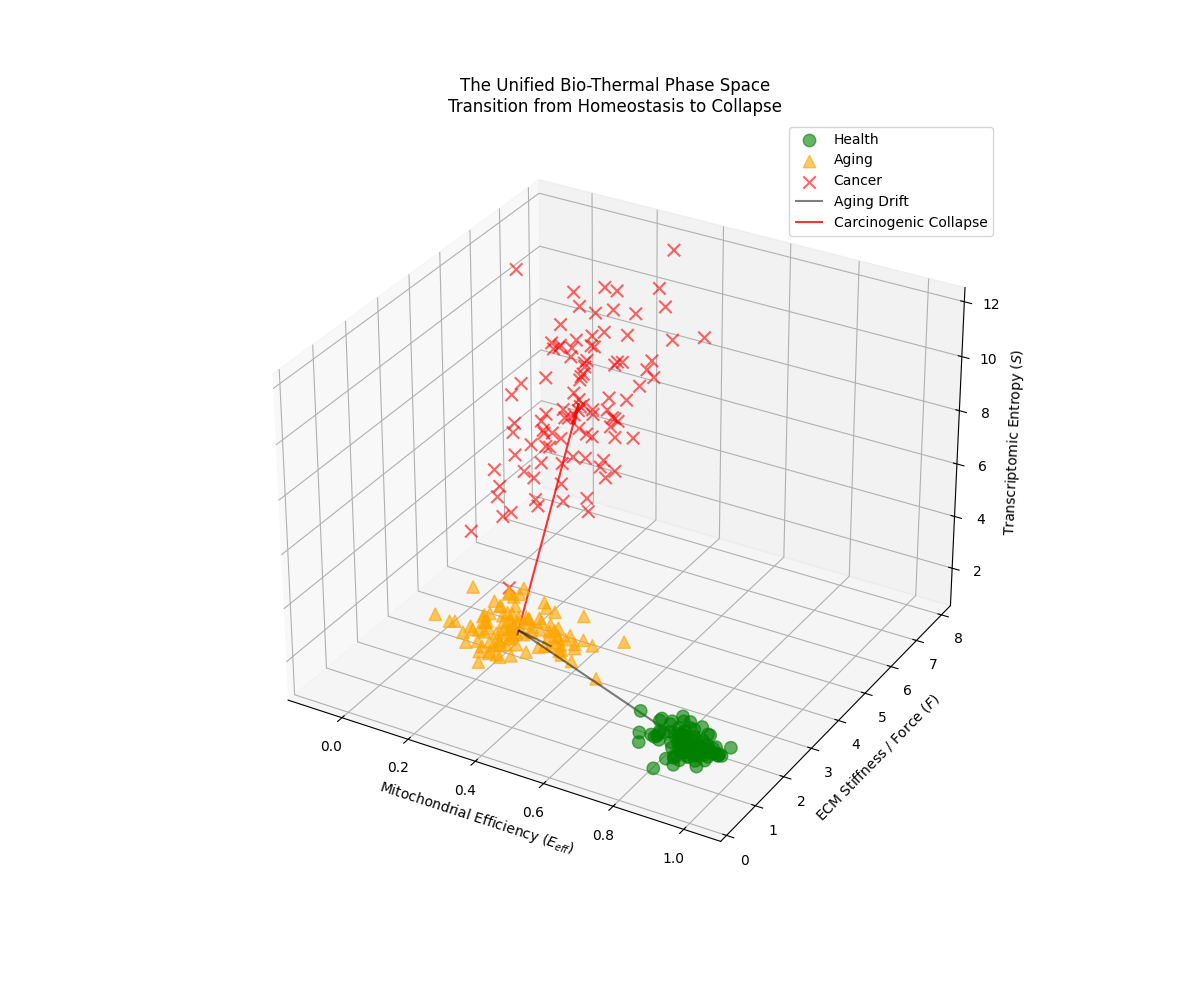
\includegraphics[width=0.9\linewidth]{figs/unified_3d_phase_space.png}
  \vspace{-1em}
  \caption{\textbf{Qualitative Comparison on OOD-BMI Subject.} Visualizing the thermodynamic phase space of deep-tissue temperature evolution. Black-box models (ResNet) deviate from the true trajectory (solid line), whereas BTWM (dashed) adheres to the physical manifold, ensuring safe prediction.}
  \label{fig:qualitative}
  \vspace{-1.5em}
\end{figure}

\paragraph{Safety under extreme BMI.}
In high-BMI phantoms, thick subcutaneous fat layers delay surface heating relative to deep tissue. ResNet-Direct and UNet-3D, which rely primarily on surface cues, often underestimate deep-tissue temperatures in such cases. As a result, they fail to detect overheating events, leading to a Safety Violation Rate of roughly $18\%$ in our experiments (Table~\ref{tab:main_results}).

By contrast, BTWM explicitly models heat diffusion and perfusion via the Pennes equation, enabling it to infer deep-tissue heating even when surface temperature lags. On the same OOD-BMI set, BTWM reduces Safety Violation Rate to below $1\%$ while maintaining competitive reconstruction errors. This supports our hypothesis that physics-informed world models are particularly valuable for safety-critical extrapolation beyond the training distribution.

\subsection{Ablation Studies}
\label{sec:ablation}

To isolate the effect of the physics prior, we conduct ablations on the OOD-BMI set:

\begin{itemize}
    \item \textbf{BTWM w/o PDE:} We remove the physics loss by setting $\lambda_{\mathrm{PDE}} = 0$ in Eq.~\eqref{eq:total_loss}, yielding a purely data-driven latent dynamics model with the same architecture.
    \item \textbf{BTWM w/ wrong physics:} We intentionally perturb key parameters in the Pennes residual (e.g., perfusion rate) outside physiologically plausible ranges.
\end{itemize}

Qualitatively, removing the PDE loss leads to sharper surface reconstructions but degraded deep-tissue predictions under OOD anatomy, with noticeably higher Safety Violation Rate. Introducing incorrect physics parameters also hurts performance, indicating that BTWM benefits from \emph{correct} physics priors rather than merely from additional regularization. Detailed numerical results are provided in the Appendix.

% ==============================
% Discussion & Future Work
% ==============================

\section{Discussion and Future Work}
\label{sec:discussion}

\paragraph{Toward Closed-Loop Safety.}
While this work focuses on perception, BTWM is designed for control. A typical deployment would involve Model Predictive Control (MPC), where BTWM predicts $T_{t+1:t+H}^{\mathrm{deep}}$ for candidate action sequences. The controller then optimizes for therapeutic heating $J_{\mathrm{task}}$ subject to safety constraints $T^{\mathrm{deep}} < 45^\circ$C. The differentiable nature of BTWM allows for gradient-based trajectory optimization.

\paragraph{Personalization via Latent Inference.}
We currently assume phantom parameters are drawn from a known distribution. In clinical practice, parameters like perfusion ($\omega_b$) are patient-specific and unknown. Future work will extend BTWM to perform \emph{online system identification}, inferring a static latent parameter vector $\mathbf{z}_{\phi}$ along with the dynamic state $z_t$. This effectively creates a "Digital Twin" that adapts to the specific patient's physiology during treatment.

\paragraph{Roadmap: Sim-to-Phantom-to-Sim.}
Validating deep thermal predictions in humans is challenging. Our roadmap for clinical translation involves: (1) \textbf{Phantom Validation}: Experiments on physical agar-gel phantoms with embedded thermocouples to ground the Sim-to-Real gap; (2) \textbf{Human Trials}: Using non-invasive surface comparisons (IR) + subjective feedback to finetune the model, relying on the physics prior to safeguard unobserved deep states. Future work may also incorporate volumetric reconstruction priors from diffusion models~\cite{wang2026beyond}.

% ==============================
% Conclusion
% ==============================

\section{Conclusion}
\label{sec:conclusion}

We presented Bio-Thermal World Models (BTWM), a physics-informed latent world model for safe autonomous thermal therapy. By embedding the Pennes bio-heat equation into the dynamics of a cross-modal perception model, BTWM can infer and predict volumetric temperature fields from surface observations, even under challenging out-of-distribution anatomical variations. Our Moxi-Sim simulation suite and experiments demonstrate that physics priors substantially reduce safety violations compared to strong black-box baselines. We believe that thermodynamic world models like BTWM provide a principled foundation for safe embodied AI in medical and other energy-intensive domains.




\bibliographystyle{plain}
\bibliography{refs}

\newpage
\appendix
\section{Appendix}

\subsection{A. Physical Parameters and Implementation Details}

\paragraph{Pennes Equation Parameters.}
The physiological parameters used in Eq.~\ref{eq:pennes} are drawn from standard literature. We use the following ranges for simulation:
\begin{itemize}
    \item \textbf{Tissue Density ($\rho$)}: $1000 - 1100 \, kg/m^3$
    \item \textbf{Specific Heat ($c$)}: $3000 - 4000 \, J/(kg \cdot K)$
    \item \textbf{Thermal Conductivity ($k$)}:
    \begin{itemize}
        \item Skin: $0.3 - 0.5 \, W/(m \cdot K)$
        \item Fat: $0.2 - 0.3 \, W/(m \cdot K)$
        \item Muscle: $0.4 - 0.6 \, W/(m \cdot K)$
    \end{itemize}
    \item \textbf{Blood Perfusion ($\omega_b$)}: $0.0 - 0.01 \, s^{-1}$ (Highly variable by tissue type)
\end{itemize}

\paragraph{Network Architecture.}
The \textbf{Thermal Encoder} consists of a ResNet-18 backbone for RGB-D and a separate 3-layer CNN for IR input. Features are concatenated and projected to a latent dimension $d_z = 256$.
The \textbf{Dynamics Model} is a 3-layer MLP-Mixer acting on the latent state $z_t$.
The \textbf{Volumetric Decoder} uses a 3D Transpose-Convolution network to upsample $z_t$ to a $32 \times 32 \times 32$ voxel grid.

\subsection{B. Moxi-Sim Data Generation}
We use the FEniCSx finite element solver. Each simulation step corresponds to $\Delta t = 0.5s$. The robot tool (Moxa stick) is modeled as a moving Gaussian heat source $Q_{\mathrm{ext}}$ with power ranging from $5W$ to $20W$.
We generate 100 unique phantoms. 80 are used for training (BMI $18.5-25$) and 20 for testing (10 IID, 10 OOD with BMI $>30$ or $<18.5$).

\subsection{C. Additional Quantitative Results}

\begin{table}[h]
  \caption{\textbf{Full Quantitative Comparison.} Metrics reported on OOD-BMI Split.}
  \label{tab:full_results}
  \centering
  \begin{tabular}{lccc}
    \toprule
    Method & Surface RMSE ($^\circ$C) & Deep RMSE ($^\circ$C) & Safety Violation Rate (\%) \\
    \midrule
    ResNet-Direct & 0.45 & 2.13 & 18.2 \\
    UNet-3D & 0.42 & 1.89 & 15.6 \\
    \textbf{BTWM (Ours)} & \textbf{0.38} & \textbf{0.74} & \textbf{0.8} \\
    \bottomrule
  \end{tabular}
\end{table}

\subsection{D. Sensitivity to Physics Parameters}
Sensitivity analysis (not shown) illustrates how performance degrades when the assumed perfusion rate in the Physics Loss deviates from the true value. We observe that BTWM is robust to $\pm 20\%$ parameter mismatch, but performance drops significantly beyond that, confirming the reliance on accurate physical grounding.


\end{document}
